\section{UML Class Diagram}
\begin{figure}[H]
    \centering
    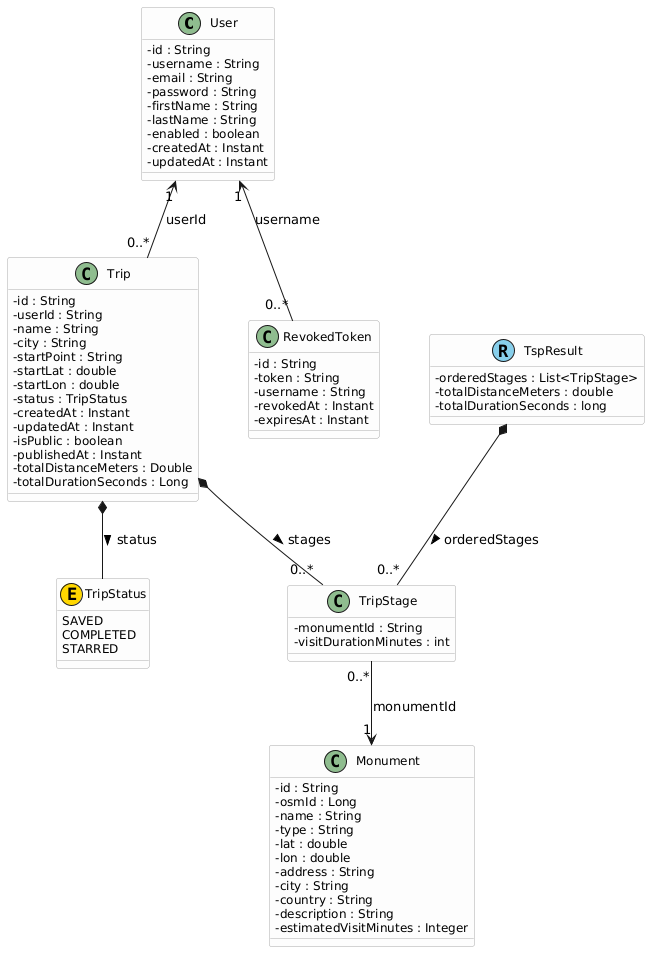
\includegraphics[width=0.85\textwidth]{Iterazione2/Diagrammi/ClassDiagram2.png}
    \caption{UML Class Diagram - Iterazione 2.}
    \label{fig:class_diagram_2}
\end{figure}

Il diagramma delle classi (\autoref{fig:class_diagram2}) mostra l'evoluzione del modello dati nella seconda iterazione. L'entità principale \texttt{Trip} è stata arricchita per poter gestire il nuovo ciclo di vita dei percorsi:
\begin{itemize}
    \item L'enumerazione \texttt{TripStatus} ora include i nuovi stati \texttt{COMPLETED} (per lo storico) e \texttt{STARRED} (per i preferiti), oltre a \texttt{SAVED} già introdotto nella fase precedente.
    \item Sono stati aggiunti gli attributi \texttt{isPublic} e \texttt{publishedAt} per gestire la visibilità dei viaggi all'interno del catalogo condiviso.
\end{itemize}
